\clearpage{\pagestyle{empty}\cleardoublepage}
\chapter{Implementazione}                %crea il capitolo
%%%%%%%%%%%%%%%%%%%%%%%%%%%%%%%%%%%%%%%%%imposta l'intestazione di pagina

Questo capitolo descrive le scelte implementative prese per la realizzazione dell'applicazione.
Il testo è arricchito da sezioni del codice sorgente, per facilitare la comprensione delle parti più complesse.

\definecolor{lightgray}{rgb}{.9,.9,.9}
\definecolor{darkgray}{rgb}{.4,.4,.4}
\definecolor{purple}{rgb}{0.65, 0.12, 0.82}
\lstdefinelanguage{JavaScript}{
  keywords={typeof, new, true, false, catch, function, return, null, catch, switch, var, if, in, while, do, else, case, break},
  keywordstyle=\color{blue}\bfseries,
  ndkeywords={class, export, boolean, throw, implements, import, this},
  ndkeywordstyle=\color{darkgray}\bfseries,
  identifierstyle=\color{black},
  sensitive=false,
  comment=[l]{//},
  morecomment=[s]{/*}{*/},
  commentstyle=\color{purple}\ttfamily,
  stringstyle=\color{red}\ttfamily,
  morestring=[b]',
  morestring=[b]",
  xleftmargin=-25pt,
  xrightmargin=-50pt,
  basicstyle=\scriptsize\sffamily
}

\section{Realizzazione della Mappa}
\subsection{Differenze con i mockup}
Durante lo sviluppo del progetto, ho apportato delle migliorie rispetto ai mockup.
Il cambiamento più significativo è stato quello di rimuovere i pin rappresentanti le varie stazioni a favore di una suddivisione in zone, ognuna delle quali delimitata da un cerchio colorato.
Il colore di ogni zona è definito dall'AQI medio mentre la grandezza dal numero di stazioni raggruppate.
Il centro di ogni cerchio è calcolato come punto medio da ogni stazione raggruppata.
Cliccando su un qualsiasi punto della mappa comparirà un pin con il nome della località, il valore AQI attuale e un grafico che mostra l'andamento della qualità dell'aria nelle ultime ore.
I pin possono essere aggiunti e rimossi in qualsiasi momento.
Premendo su un pin viene mostrato il menù a scomparsa per personalizzare la sonificazione.
Tralasciando qualche dettaglio grafico e di scelta dei colori, il menù è simile a quello presente nel mockup; una differenza volta a migliorare l'esperienza utente è stata quella di pre-impostare l'intervallo di tempo per la sonificazione a quello mostrato nel pin.
Al fine di permettere all'utente di effettuare più sonificazioni contemporaneamente, il player video è stato rimosso dalla pagina.
Ad ogni richiesta di sonificazione, viene mostrata in basso a destra una notifica cliccabile, che permette di aprire la simulazione in una nuova scheda del browser.
I colori utilizzati per i grafici, i cerchi e le notifiche riprendono quelli stabiliti dallo standard AQI \ref{tab:aqi}. La schermata finale è rappresentata in Figura \ref{fig:schermata}.
\begin{figure}[h]
  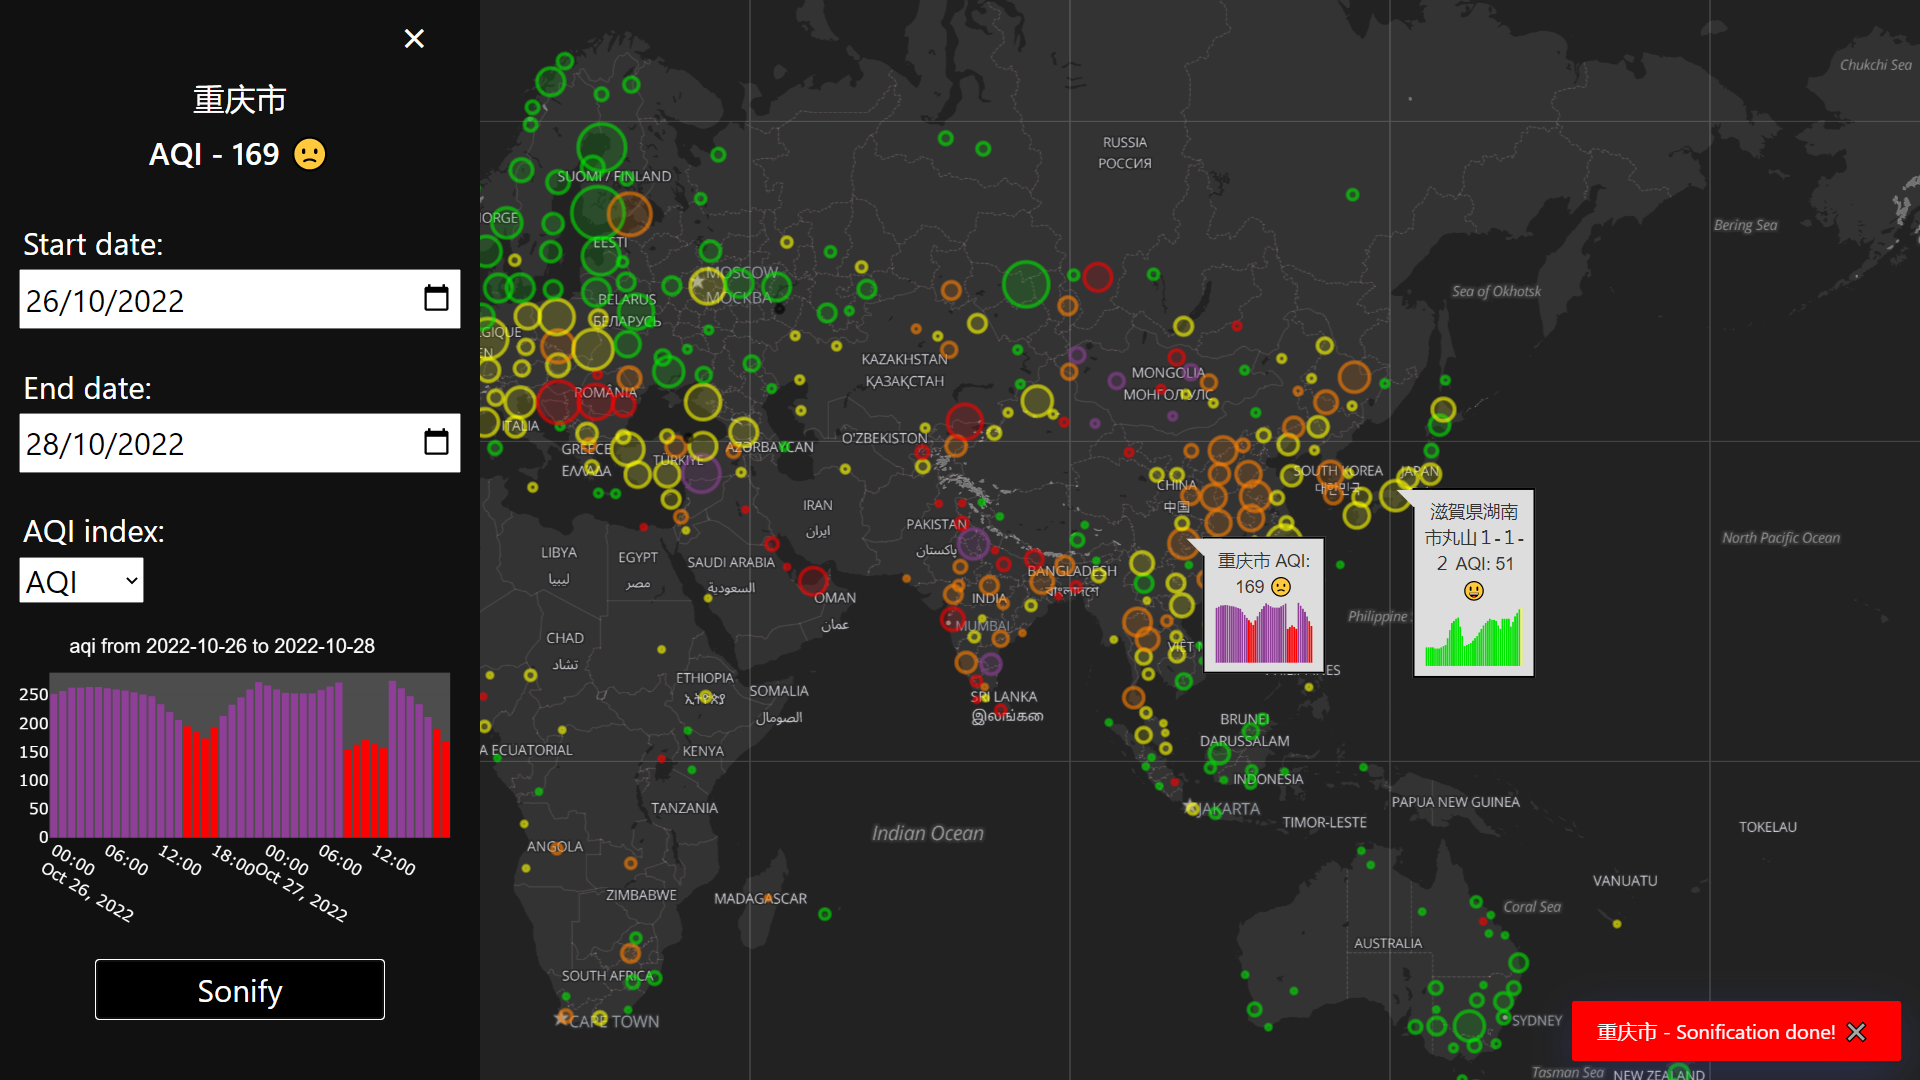
\includegraphics[width=\linewidth]{img/schermata.png}
  \caption{La schermata e le varie componenti}
  \label{fig:schermata}
\end{figure}
\subsection{Dettagli implementativi}
\subsubsection{Generazione dei cerchi}
La preparazione della schermata avviene in diverse fase consecutive.
Per prima cosa, tramite la libreria Leaflet, la mappa viene creata e visualizzata nella pagina.
Immediatamente dopo, tramite una chiamata all'API di AQIcn, vengono scaricati i dati relativi a tutte le stazioni di rilevazione presenti.
La visualizzazione delle zone circolari è affidata alla funzione load circles (listato ~\ref{lst:loadCircles}), che prende come unico parametro un oggetto JSON \cite{json}, contenente i dati delle stazioni.
La funzione divide il mondo in un totale di 4900 zone, 70 in altezza e 70 in larghezza, ognuna identificata da un indice univoco.
Per ogni stazione di ricerca, viene calcolato l'indice della zona a cui appartiene e viene inserita in un'apposita struttura dati.
\begin{lstlisting}[language=Javascript,caption={Suddivisione in zone delle stazioni.},label={lst:loadCircles}]
// get chunk unique index based on lat, lng
function get_chunk_idx(lat, lng, chunks_per_dim) {
    let lat_chunk = Math.floor((lat + 90) / 180 * chunks_per_dim);
    let lng_chunk = Math.floor((lng + 180) / 360 * chunks_per_dim);
    return lat_chunk * chunks_per_dim + lng_chunk;
}

// define chunk size
let chunks = {};
let chunks_per_dim = 70;   

// load chunks
for(let pin of data) {
    // ignore stations with no data
    if(pin.aqi == '-') continue;
    let lat = pin.lat;
    let lng = pin.lon;
    let chunk_idx = get_chunk_idx(lat, lng, chunks_per_dim);
    if(!(chunk_idx in chunks)) 
        chunks[chunk_idx] = [pin];
    else 
        chunks[chunk_idx].push(pin);
}
\end{lstlisting}
In seguito alla suddivisione in zone, per ognuna di queste viene calcolato il valore AQI e il punto medio delle stazioni raggruppate; 
in base a queste informazioni, viene disegnato un cerchio di colore e grandezza appropriati. Eventuali zone vuote vengono ignorate.


\subsubsection{Implementazione dei marker personalizzati}
Cliccando sulla mappa, viene eseguita la funzione map inspect (listato ~\ref{lst:mapInspect}).
Per prima cosa la funzione ottiene la latitudine e la longitudine del punto cliccato e, tramite reverse geocoding, ottiene il nome della località.
L'esecuzione passa in seguito alla funzione create marker che, da un set di coordinate e un nome, crea un marker personalizzato (listato ~\ref{lst:createMarker}).
La funzione si occupa, inoltre, di ottenere lo storico delle ultime rilevazioni AQI della zona, eseguendo una chiamata all'API di weatherbit.io, questi dati
vengono utilizzati in seguito per creare il grafico che compare nel pin.
Per rimuovere un pin, è sufficiente cliccare con il tasto destro del mouse, o effettuare una pressione prolungata se da mobile.
La struttura di un marker è un'estensione di quella default offerta da leaflet, sono state aggiunte le informazioni relative alla posizione geografica e all'ultima rilevazione AQI avvenuta, al fine di semplificare la gestione dei dati (listato ~\ref{lst:markerextension}).
\begin{lstlisting}[language=Javascript,caption={La struttura di un marker personalizzato.},label={lst:markerextension}]
// custom marker extension, values are placeholders
myAqiMarker = L.Marker.extend({
    options: {
        aqi: 0,       // last aqi value detected
        location: '', // location name
        lat: 0,       // latitude
        lng: 0        // longitude
    }
});
\end{lstlisting}

\begin{lstlisting}[language=Javascript,caption={La funzione map inspect.},label={lst:mapInspect}]
async function map_inspect(event) {

  // event consiste nelle informazioni relative all'evento di pressione sulla mappa
  let latlng = event.latlng;
  let lat = latlng.lat
  let lng = latlng.lng
  // reverse geocoding to get location name
  await geocodeService.reverse().latlng(event.latlng).run(async function (error, result) {

      // get address
      let add = result.address;
      let location = add.City || add.LongLabel;
      // add marker
      create_marker(lat, lng, location);

  });

}
\end{lstlisting}


\begin{lstlisting}[language=Javascript,caption={La funzione create marker.},label={lst:createMarker}]
async function create_marker(lat, lng, location) {
    
    // load history
    get_today_history(lat, lng).then(async(history) => {

        // get the history
        let id = String(Date.now());
        let aqis = await history.get_index('aqi');
        let time = await history.get_index('timestamp_local');
        let aqi = aqis[aqis.length - 1];

        new aqiMarker([lat, lng], {

            // custom marker label
            icon: L.divIcon({
                className: 'my-div-icon',
                html:
                    `<div class="speech-bubble">
                        ${location} AQI: ${aqi} ${get_emoji(aqi)}
                        <img class="aqi_preview" id="${id}"></img>
                    </div>`,
            }),
    
            // additional marker info
            location: location,
            aqi: aqi,
            lat: lat,
            lng: lng,
    
        }).addTo(layerGroup).on('click', load_offcanvas).on('contextmenu', function(e) { map.removeLayer(this); });
    
        // create graph inside the marker
        create_small_graph(aqis, time, id);

    });
    
}
\end{lstlisting}

\subsubsection{Utilizzare il geocoding}
All'utente è data la possibilità di ispezionare una località specificandone il nome, l'indirizzo o la posizione geografica.
La ricerca vera e propria è delegata all'API Esri di ArcGIS, che restituisce una lista di possibili risultati mostrati sotto la casella di testo.
Al click di uno di questi, dall'evento, viene estratto il nome del luogo, la latitudine e la longitudine, con questi parametri, viene chiamata la funzione map inspect, spiegata precedentemente.


\lstloadlanguages{Python}
\lstset{
  language=Python,
  basicstyle=\scriptsize\sffamily,
  stringstyle=\color[HTML]{933797},
  commentstyle=\color[HTML]{228B22}\sffamily,
  emph={[2]from,import,pass,return}, emphstyle={[2]\color[HTML]{DD52F0}},
  emph={[3]range}, emphstyle={[3]\color[HTML]{D17032}},
  emph={[4]for,in,def}, emphstyle={[4]\color{blue}},
  showstringspaces=false,
  breaklines=true,
  prebreak=\mbox{{\color{gray}\tiny$\searrow$}},
  xleftmargin=-25pt,
  xrightmargin=-50pt,
}

\subsubsection{Personalizzare la sonificazione}
Al click del marker, viene mostrato un menù a scomparsa che permette di personalizzare la sonificazione (Figura \ref{fig:schermata}).
I dati, quale il nome della località, l'intervallo di date iniziale e l'ultima rilevazione AQI effettuata, sono caricati direttamente a partire dal marker che ha chiamato la funzione.
Al cambiamento di ogni elemento presente nel form di personalizzazione è associato una funzione che valida i dati inseriti e, in caso di successo abilita il pulsante di conferma e aggiorna il grafico di anteprima (listato ~\ref{lst:formChange}).
In aggiunta, in caso di dati validi, le informazioni riguardanti la sonificazione vengono caricati in una struttura dati denominata sonification data, che verrà usata come payload della richiesta di sonificazione.

\begin{lstlisting}[language=Javascript,caption={La funzione che gestisce il cambiamento di un elemento del form.},label={lst:formChange}]
async function load_index(){

  // load useful data from form
  let start_date  = $("#offcanvas_start_date").val();
  let end_date    = $("#offcanvas_end_date").val();
  let lat         = $("#offcanvas_aqi").attr("data-lat");
  let lng         = $("#offcanvas_aqi").attr("data-lng");
  let index       = $("#offcanvas_index").val();
  
  get_history(lat, lng, start_date, end_date, index).then(async (history) => {

    let aqis = await history.get_index(index);
    let time = await history.get_index('timestamp_local');
    create_graph_image(aqis, time, "offcanvas_plot", `${index} from ${start_date} to ${end_date}`);
    $("#offcanvas_btn_sonify").show();

    sonification_data = {
      idx: index,
      data: aqis,
      days: time,
      location: $("#offcanvas_location").text()
    }

  }).catch(async (error) => {
      
    // if form data is invalid, or api call fails, hide sonify button
    $("#offcanvas_btn_sonify").hide();
    $("#offcanvas_plot").attr("src", "");
    console.log(error);

  });

}
\end{lstlisting}

\subsubsection{Gestire lo storico}
Lo storico delle rilevazioni AQI è gestito nel file aqi api.js.
Per ottenere lo storico, è necessario creare una nuova istanza della classe History, passando come parametri la latitudine e la longitudine della zona di interesse e l'intervallo di date (listato ~\ref{lst:history}).
Una volta ottenuto l'oggetto, tramite la funzione get index, è possibile ottenere un array contenente i valori di un indice di interesse, quali il PM10, il PM2.5, l'O3, ecc.
\begin{lstlisting}[language=Javascript,caption={La classe History.},label={lst:history}]
function History(lat, lng, start_date, end_date) {
    this.lat = lat;
    this.lng = lng;
    this.start_date = start_date;
    this.end_date = end_date;
}

History.prototype.load = async function() {
    let request = `https://api.weatherbit.io/v2.0/history/airquality?lat=${this.lat}&lon=${this.lng}&start_date=${this.start_date}&end_date=${this.end_date}&tz=local&key=${weatherbit_key}`;
    let response = await fetch(request);
    let resp_data = await response.json();
    this.data = resp_data.data;
}

History.prototype.get_index = async function(index) {
    let arr = this.data.map((item) => item[index]);
    return arr.reverse();
}
\end{lstlisting}

\subsubsection{Tutorial}
Al fine di migliorare la user experience, ho inserito un semplice tutorial che spiega come utilizzare l'applicazione.
Il tutorial consiste in dei messaggi che vengono mostrati nella parte inferiore dello schermo (Figura \ref{fig:tutorial}).
Ogni messaggio rimane in attesa del completamento di una determinata azione, al compimento di questa, il messaggio viene nascosto e viene mostrato il successivo.
Solo seguendo il tutorial, l'utente può effettuare la prima sonificazione.


\begin{figure}[h]
  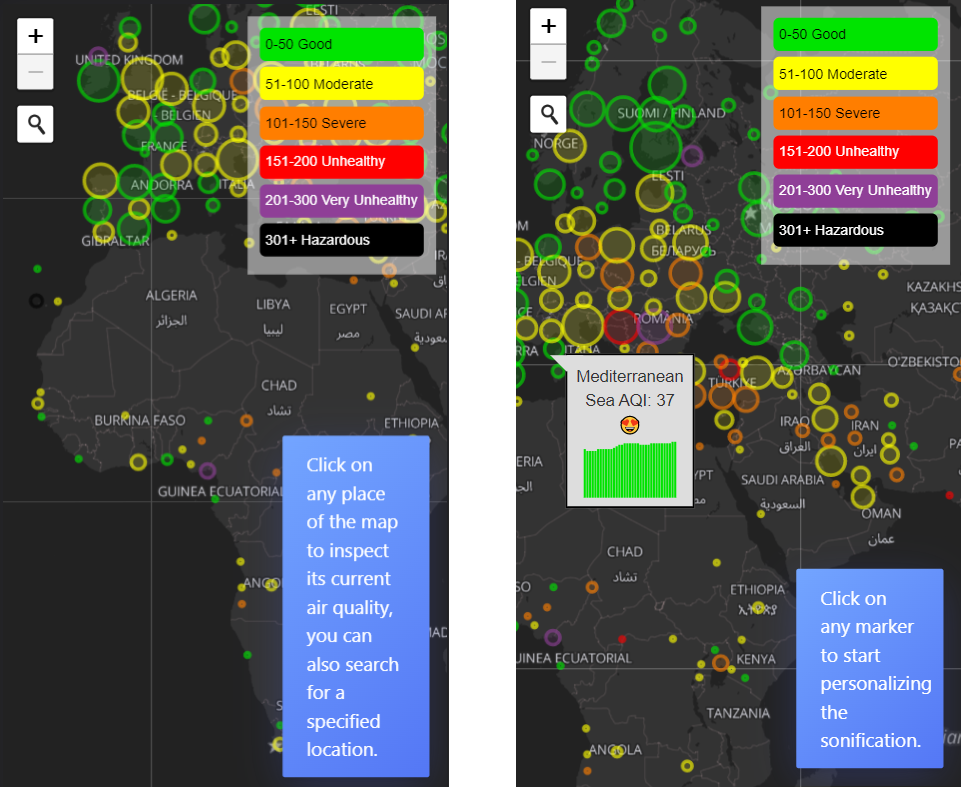
\includegraphics[width=\linewidth]{img/tutorial.png}
  \caption{Due fasi del tutorial, in particolare, quelle che richiedono all'utente di aggiungere e cliccare un marker.}
  \label{fig:tutorial}
\end{figure}

\newpage


\section{Implementazione del server}
Il server è in grado di ricevere richieste di tre tipi, in base al percorso di questa.
Per ottenere la pagina web interagibile, è possibile effettuare una richiesta GET al percorso / (root del server), da qualsiasi browser web.
Una volta selezionata la località, l'indice da sonificare, e l'intervallo di date, tramite il bottone sonifica viene eseguita una richiesta POST al percorso /sonify; i dati citati precedentemente sono inviati in formato JSON (listato ~\ref{lst:sonify}).
Questa richiesta richiama, in un processo secondario, lo script sonify.py; al suo completamento, il server legge i byte del file video generato e li restituisce al client.
Cliccando sulla notifica di avvenuta sonificazione, il client effettua una richiesta GET al percorso /video, che apre, in una nuova scheda, una schermata con il video riproducibile.

\begin{lstlisting}[language=Python,caption={La funzione che gestisce la richiesta /sonify.},label={lst:sonify}]
class SonifyRequest(BaseModel):
  data:   list = Field(..., example=[121, 140, 150, 51, 67, 18])
  days:   list = Field(..., example=["2021-01-01T00:00:00", "2021-01-01T00:00:01"])
  idx:    str # (AQI, PM25, PM10...)
\end{lstlisting}



\section{Sonificazione}
Di seguito vengono approfondite le scelte implementative per quanto riguarda la realizzazione della sonificazione vera e propria.
Le sezioni di codice successive fanno ampimente uso di due funzioni di utility, in grado di cambiare un valore da un intervallo di valori ad un altro (listato ~\ref{lst:utils}).

\begin{lstlisting}[language=Python,caption={Funzioni utility.},label={lst:utils}]
def map_value(value, in_min, in_max, out_min, out_max):
  # handles rare case where minium AQI and maximum AQI are the same
  if in_min == in_max:
      return (out_min + out_max) / 2
  return (value - in_min) * (out_max - out_min) / (in_max - in_min) + out_min

def map_value_int(value, in_min, in_max, out_min, out_max):
  return math.floor(map_value(value, in_min, in_max, out_min, out_max))
\end{lstlisting}



\subsection{Aspetti dell'inquinamento Sonificati}
Prima di progettare il sistema sonificativo, ho individuato le caratteristiche dei dati che volevo rappresentare:
le componenti di maggiore importanza sono l’andamento temporale dell'inquinamento e l'inquinamento residuo.
Queste due tracce sono accompagnate da un sottofondo sonoro, che audifica la forma del grafico AQI.
\subsubsection{L'andamento dell'inquinamento}
L'andamento temporale è rappresentato dalle varie rilevazioni nel tempo, siccome è un valore che tende a cambiare rapidamente nel tempo, ha richiesto un approccio di sonificazione dinamico.
La scelta delle note utilizzate per rappresentare questo dato è molto semplice: più il valore dell'inquinamento è alto, più la nota è grave.
\subsubsection{L'inquinamento residuo}
L'inquinamento residuo consiste nel valore di rischio per la salute che si protrae nel tempo in seguito ad una giornata particolarmente inquinata.
A differenza della rilevazione AQI vera e propria, i cui valori possono variare drasticamente da un momento all'altro, l'accumulo di residuo si distingue in fasi di crescita e di diminuzione, in funzione a come si è comportato l'inquinamento nel corso della giornata \cite{residue}.
Per le fasi di crescita ho usato delle note veloci che si alzano di tonalità, mentre per la fase di diminuzione le stesse note sono ripetute con meno frequenza, e tendono ad abbassarsi nel tempo.
\subsubsection{Gestire il volume}
Un aspetto molto rilevante che ho attribuito a queste due tracce sta nella miscela dei loro volumi: più il valore dell'inquinamento tende ad alzarsi, più il suo volume si abbassa per lasciare spazio alla traccia dell'inquinamento residuo, che invece tende a crescere.
\subsubsection{L'applicazione della teoria musicale}
Per accentuare l'effetto della crescita e della diminuzione dell'inquinamento residuo, le note della traccia seguono una scala: più l'inquinamento è alto più le note sono acute.
Ho deciso di utilizzare una scala maggiore. Siccome le tonalità maggiori sono note per la loro positività, ho introdotto delle dissonanze in base al peggioramento della qualità dell'aria, volte a spezzare questa armonia.
Una dissonanza è una nota “fuori contesto” rispetto alla scala o all'accordo che si sta suonando; se inserita all'interno di una scala maggiore, sempre positiva e armoniosa, la dissonanza crea un effetto improvviso di tensione \cite{dissonance}.
Ho posto le dissonanze ad intervalli regolari nella scala in base al livello di inquinamento: più questo è alto, più le dissonanze sono frequenti e di maggior intensità.




\subsection{Esportare una traccia audio}
Prima di analizzare la logica secondo la quale ogni traccia viene creata, è importante capire come il sistema esporta gran parte di queste.
L'esportazione e la sintesi delle traccie audio MIDI avvengono tramite la classe AudioExporter.
La classe prende come parametri di costruzione le metriche di pentagramma per la traccia, quali il bpm e la suddivisione del tempo.
La funzione di classe volta alla sintesi vera e propria accetta come argomenti una lista di note, un nome per la traccia, l'indice di uno strumento General MIDI e una lista di effetti audio VST3 da applicare.
Le note sono delle strutture dati che contengono le informazioni necessarie per descrivere un evento MIDI (listato ~\ref{lst:note}).

\begin{lstlisting}[language=Python,caption={Composizione di una nota.},label={lst:note}]
note = {"note": 44,           # indice della nota
        "time": start_time,   # il tempo di inizio, in battiti 
        "duration": duration, # la durata, in quarti di battito
        "volume": vol}        # il volume 0 - 100, valore facoltativo
\end{lstlisting}
A partire da una lista di note, viene generato un file MIDI .mid, questo viene sintetizzato un un file .wav da timidity++, tramite una chiamata di sistema.
In seguito, il file sintetizzato viene caricato sotto forma di array di campioni stereo, al quale vengono applicati gli effetti audio.



\subsection{Traccia principale e accordi - Lead}
La traccia principale sonifica l'indice di qualità dell'aria.
Questa traccia si basa su una scala maggiore ed è caratterizzata da una nota per rilevazione, presenta un timbro dolce.
La traccia è principalemente presente negli istanti nei quali la qualità dell'aria è ottimale, quando questa peggiora,
il suo volume tende ad abbassarsi lasciando spazio alla traccia di residuo.
Ogni nota è caratterizzata da una tonalità ed un volume che dipendono dalla gravità dell'AQI rispetto al valore maggiore e minore registrato.
Alle note del Lead vengono affiancati degli accordi ripetuti ad ogni battuta, l'ottava di ognuno di questi è determinata dalla media di quattro rilevazioni consecutive. In (listato ~\ref{lst:lead}) viene mostrala la generazione del lead.

\begin{lstlisting}[language=Python,caption={Generazione della traccia principale.},label={lst:lead}]
def get_lead(data, voicing):

  voicing = voicing[::-1]
  n_notes = len(voicing)
  best    = min(data)
  worst   = max(data)
  notes   = []

  for i in range(len(data)):
      aqi       = data[i]
      vol       = 75 if aqi < MIN_THRESH else map_value_int(aqi, best, worst, 50, 25)
      note_idx  = map_value_int(aqi, best, worst, 0, n_notes - 1)
      notes.append({"note": voicing[note_idx], "time": i, "duration": 1, "volume": vol })

  return notes

\end{lstlisting}

\newpage

\subsection{Sonificazione del residuo}
Il procsso relativo alla creazione della traccia di residuo è implementato nel file residue.py.
La funzione prende come parametro l'array di rilevazioni AQI, e restituisce una lista di note MIDI.
\subsubsection{Individuare i picchi di residuo}
La prima cosa svolta in questo procedimento è individuare l'andamento del residuo.
Per raggiungere questo scopo, all'array di rilevazioni viene affiancato un array di residuo riempito con il seguente criterio:
Quando viene rilevato un valore AQI non ottimale, il residuo raggiunge tale valore, altrimenti, il residuo viene diminuito di un valore costante.
\subsubsection{Generazione delle note}
Le note sono generate in base agli intervalli di crescita e diminuzione del residuo.
La sonificazione segue questo criterio: appena viene rilevata una fase di crescita, viene creato un arpeggio di note di tonalità ascendenti, che si protrae fino alla fine di questa.
La frequenza è di quattro note per rilevazione, e le tonalità sono uniformemente distribuite tra le note della scala selezionata; il volume è ascendente.
Alla fase della crescita segue un'eventuale fase di diminuzione, caratterizzata da un arpeggio di note di tonalità e volume discendenti con frequenza di due note a rilevazione. La fase
di discesa si protrae fino alla completa risanazione dell'aria o fino all'inizio di un nuovo intervallo di crescita.
Tramite questa strategia, sono riuscito a differenziare gli arpeggi tra le crescite improvvise di inquinamento e quelle più progressive.
Durante le fasi di crescita e diminuzione del residuo, sono posizionate delle dissonanze in base alla gravità del valore (listato ~\ref{lst:residue}).

\newpage

\begin{lstlisting}[language=Python,caption={Implementazione dell'algoritmo di residuo.},label={lst:residue}]
  # iterate len(residue) *4 times
  # each value in residue is a beat, each beat has 4 notes
  for i in range(len(residue) * 4):

      # check if a new beat has started
      if i % 4 == 0:
          idx = i // 4
          res = residue[idx]
          vol = map_value_int(res, 0, max_res, 0, 100)
          last_res = residue[idx-1] if idx > 0 else 0

          # detect rising slope
          if res > last_res and res >= MIN_THRESH and idx > target_idx:
              # find the end of the rising slope
              target_idx  = get_rising_end(idx)
              target_res  = residue[target_idx]

              # arpeggio lenght
              arp_len     = map_value_int(target_res, 0, max_res, 0, len(voicing)-1)
              # initial note index (mapped residue to len(voicing))  
              init_start  = map_value_int(res, 0, max_res, 0, len(voicing) - 1)       
              # actual number of notes (in pows of 4)
              init_notes  = math.ceil(target_idx - idx + 1) * 4                       
              # indexes of notes of initial arp (not actual notes)
              init_idxs   = np.linspace(init_start, arp_len, init_notes, dtype=int)   
              # broadcasting indexes to notes
              init_arp    = [voicing[pos] for pos in init_idxs]                       
              init_done   = False
              init_ptr    = 0

      # get dissonation
      dissonation = get_dissonation(i, res, max_res)

      # before falling, a full complete init arpeggio is always played
      if init_done == False:
          notes.append({"note": init_arp[init_ptr] + dissonation, "time": duration * i, "duration": duration, "volume": vol })
          if init_ptr >= len(init_arp) - 1:
              init_done = True
          else:
              init_ptr += 1
      # falling, note on 1,0,1,0
      elif res >= MIN_THRESH and i % 2 == 0:
          note_idx = map_value_int(res, 0, max_res, 0, len(voicing) - 1)
          notes.append({"note": voicing[note_idx] + dissonation, "time": duration * i, "duration": duration, "volume": vol })

\end{lstlisting}


\begin{figure}[h]
  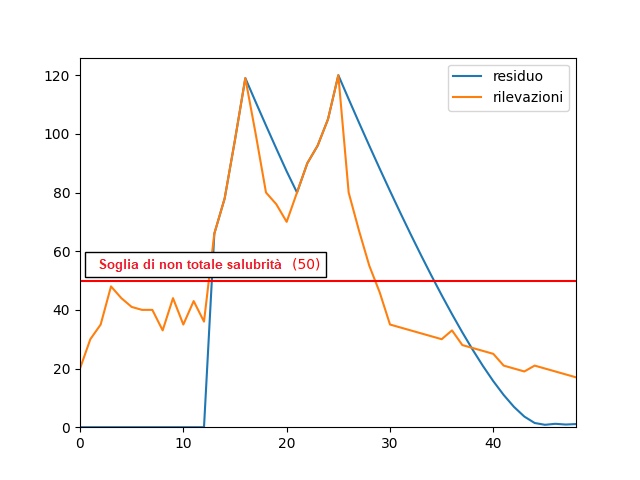
\includegraphics[width=\linewidth]{img/residue.png}
  \caption{L'andamento del residuo con delle possibili rilevazioni.}
  \label{fig:residue}
\end{figure}








\subsection{Generazione del Sub Bass di sottofondo} 
La traccia di sub-bass viene generata tramite un algoritmo implementato nei file sub e wave buffer.
Questa è l'unica traccia che viene effettivamente sintetizzata, e non è basata su note MIDI.
L'unico parametro di cui il processo ha bisogno è l'array di dati relativi alle varie rilevazioni, l'oggetto prodotto è un array di campioni audio stereo.
\subsubsection{Suddivisione dei dati in intervalli}
Il primo passo che questo sottosistema svolge è quello di dividere tutte le rilevazioni in sottointervalli di AQI consecutivi non ottimali.
Per ogni sottointervallo, ne viene indicato l'indice di inizio e quello di fine.
\subsubsection{Generazione delle WaveTable}
In seguito alla suddivisione, per ogni intervallo viene generata una WaveTable.
Per prima cosa viene prelevato il sub-array di dati relativo all'intervallo, in segutio, tramite la classe specificata in wavebuffer.py (listato ~\ref{lst:wavebuffer}), viene creato l'array di campioni wavetable.
Partendo dai dati grezzi, ovvero le sole rilevazioni AQI, il primo passo che la classe svolge è quello di aggiungere all'array una sua copia negativa, in modo da rispettare l'ampiezza massima e minima di un segnale audio.
In seguito vengono aggiunti, tramite interpolazione periodica, tanti punti quanti sono i campioni che la WaveTable deve contenere, nel mio caso, 8192.
Ho scelto l'interpolazione periodica per fare combaciare sempre il primo campione con l'ultimo, rendendo l'onda effettivamente continua.
A seguito dell'interpolazione, ogni campione viene attenuato, ogni valore nella wavetable viene quindi mappato in un numero compreso tra 1 e -1.
Infine, al segnale viene applicato un filtro "Sample n Hold": un circuito che, preso come input un segnale, ne diminuisce la frequenza di campionamento.
L'intervallo di campionamento per il Sample n Hold è stabilito dall'AQI medio, più è alto, più l'onda perde di segnale e risulta invasiva.
\\
\begin{figure}[h]
  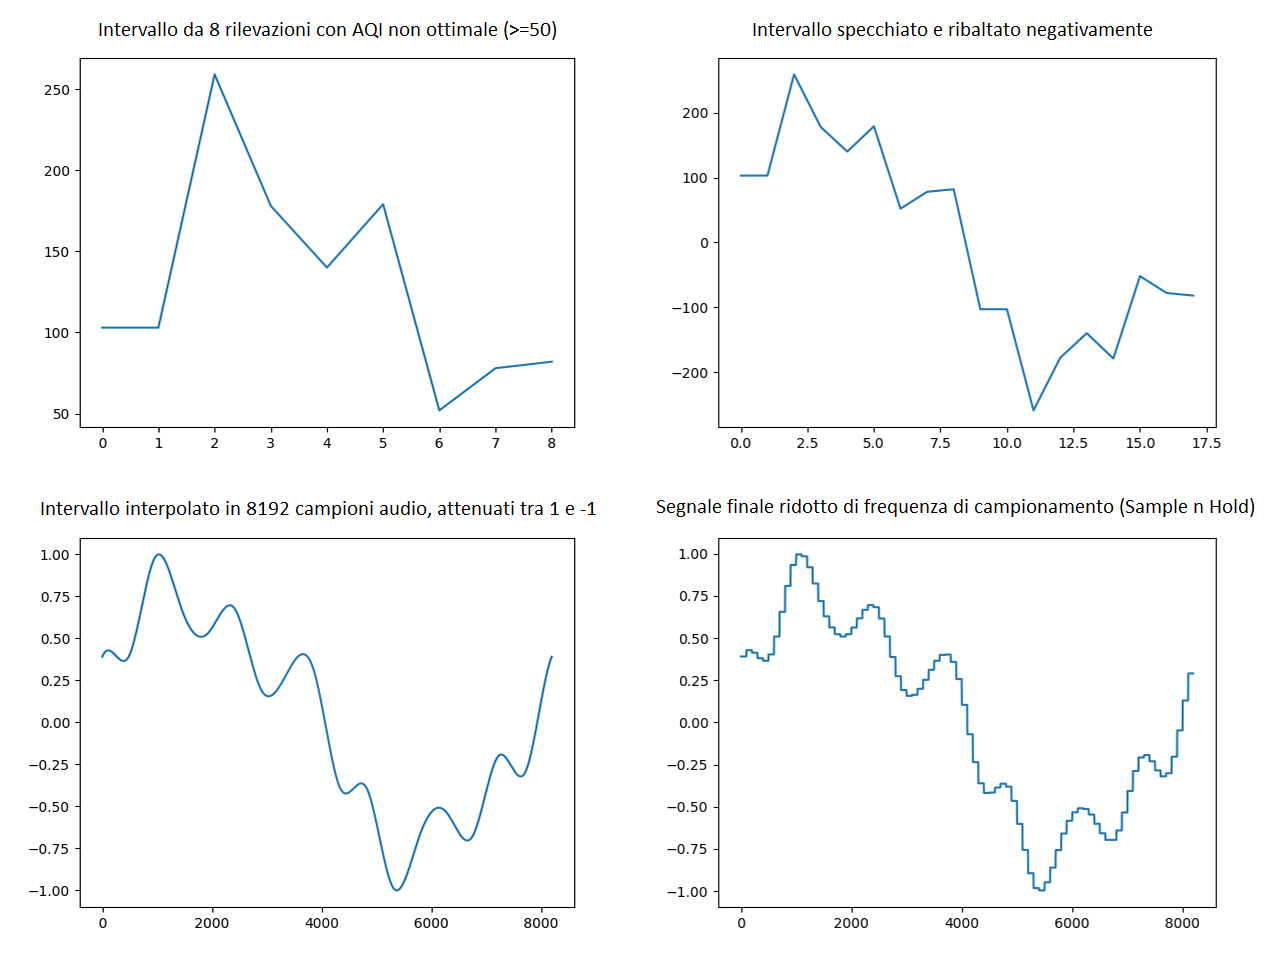
\includegraphics[width=\linewidth]{img/waves.png}
  \caption{Le fasi della generazione di una WaveTable.}
  \label{fig:wave_sub}
\end{figure}

\newpage

\begin{lstlisting}[language=Python,caption={La classe che si occupa della generazione di WaveTable.},label={lst:wavebuffer}]
class WaveBuffer(object):

  def __init__(self, buffer):
      self.buffer = buffer

  # map every value between amp_targer and amp_target * -1
  def amplify(self, amp_target = 1):
      max_item = max(self.buffer)
      amp = amp_target / max_item
      return WaveBuffer([sample * amp for sample in self.buffer])

  # add a copy of the buffer with inverted values
  def mirror_extend(self):
      half_len = len(self.buffer)        
      mirrored = self.buffer + self.buffer
      return WaveBuffer([mirrored[i] if i < half_len else mirrored[i] * -1 for i in range(len(mirrored))])

  # interpolate buffer to given point number (default is 8192)
  def interpolate(self, points = WAVETABLE_SIZE): # 8192 = default wavetable size
      y = self.buffer
      x = np.arange(len(y))
      spl = splrep(x, y, per=True)
      newx = np.linspace(0, len(y)-1, points)
      return WaveBuffer(splev(newx, spl))

  # apply a sample and hold filter to the buffer
  def quantize(self, samples):
      return WaveBuffer([self.buffer[math.floor(i / samples) * samples] for i in range(len(self.buffer))])

  # return the buffer
  def get_buffer(self):
      return self.buffer
\end{lstlisting}



\subsubsection{Preparazione dei modificatori di volume: LFO, Enveloper}
Prima di passare alla sintesi vera e propria, il sottosistema definisce gli elementi necessari per l'andamento dinamico del volume.
Gli elementi sono l'LFO e l'Enveloper.
In questa sonificazione, l'LFO appare come una funzione sinusoidale periodica che oscilla tra 0.5 e 1.5, i valori che andranno a moltiplicarsi al volume.
L'LFO viene restituito sotto forma di lambda dalla seguente funzione (listato ~\ref{lst:lfo}).

\begin{lstlisting}[language=Python,caption={Generazione dell'LFO.},label={lst:lfo}]
def compute_LFO(min, max, samp_period): 
    # samp_period = distanza in campioni tra i picchi della funzione
    freq = 1 / (samp_period / SAMPLE_RATE)
    period = SAMPLE_RATE / freq
    half = (max - min) / 2
    return lambda x: math.sin(2.0 * math.pi * (x) / period) * half + half + min
\end{lstlisting}
L'enveloper appare come una semplice funzione che, preso come parametro un array di campioni, ne attenua l'inizio e la fine (listato ~\ref{lst:enveloper}).

\begin{lstlisting}[language=Python,caption={La funzione Enveloper.},label={lst:enveloper}]
def envelope_buffer(buffer):

  nsamples    = len(buffer)
  attack_s    = nsamples * 0.1
  decay_s     = nsamples * 0.1

  for i in range(nsamples):
      if i < attack_s:
          buffer[i] *= map_value(i, 0, attack_s, 0, 1)
      if i > nsamples - decay_s:
          buffer[i] *= map_value(i, nsamples - decay_s, nsamples, 1, 0)

  return buffer
\end{lstlisting}

\subsubsection{Sintesi}
Si può passare alla funzione di sintesi vera e propria (listato ~\ref{lst:audio_buffer}).
La prima cosa svolta dalla funzione è definire le metriche della traccia, quali il tempo, il numero di note per intervallo, la frequenza di campionamento e la tonalità che si vuole rappresentare.
Per ogni intervallo viene generato un buffer audio, questi verranno poi concatenati in un unico array.
Ogni intervallo è composto da più rilevazioni, ognuna delle quali verrà sonificata con quattro note; il volume e la durata di ogni nota è definita dalla gravità dell'AQI della rilevazione.
I campioni inseriti nel buffer vengono presi dalla WaveTable relativa all'intervallo.
Il valore di ogni campione viene moltiplicato per il volume e per il relativo valore della funzione LFO.
Al fine nascondere le discontinuità delle onde nelle note suonate, il buffer di ognuna di queste viene processato dalla fuzione Enveloper, che attenua i primi e gli ultimi campioni.


\begin{lstlisting}[language=Python,caption={Generazione del buffer audio.},label={lst:audio_buffer}]
def get_wav(data, intervals, wavetables, B):

  B_PER_SEC   = BPM / 60                  # beats per second
  SECONDS     = B / B_PER_SEC             # total track seconds
  SAMPLES     = SECONDS * SAMPLE_RATE     # total track samples

  NOTE_FREQ   = 65.41                                         # C2
  NOTES_PER_B = 4                                             # notes per beat
  STEP        = (NOTE_FREQ * WAVETABLE_SIZE) / SAMPLE_RATE    # wavetable step
  SAMPS_PER_N = int(SAMPLE_RATE / B_PER_SEC / NOTES_PER_B)    # samples per note

  LFO         = compute_LFO(0.5, 1.5, SAMPLE_RATE // B_PER_SEC)
  buff        = np.zeros(int(SAMPLES))
  lfo_ptr     = 0

  # iterate over intervals
  for interval_idx in range(len(intervals)):

      interval    = intervals[interval_idx]
      start, end  = interval[0], interval[1]
      wavetable   = wavetables[interval_idx]

      # iterate over measurements in interval
      for data_idx in range(start, end):

          aqi = data[data_idx]
          vol = map_value(aqi, MIN_THRESH, MAX_THRESH, 0, 0.05)
          dur = map_value_int(aqi, MIN_THRESH, MAX_THRESH, SAMPS_PER_N // 4, SAMPS_PER_N)

          # each measurements has 4 consecutive notes
          for note_idx in range(NOTES_PER_B):

              note_start  = math.floor((data_idx + (note_idx / NOTES_PER_B)) * (SAMPLE_RATE / B_PER_SEC))
              note_buff   = np.array([wavetable[math.floor(i * STEP) % WAVETABLE_SIZE] * vol * LFO(i + lfo_ptr) for i in range(dur)])
              env_buffer  = envelope_buffer(note_buff)
              lfo_ptr     += dur
              buff[note_start:note_start + dur] += env_buffer

  return buff
\end{lstlisting}

\section{Merging delle tracce}
Una volta pronti gli array di tutte le traccie audio, questi vengono uniti in un'unica lista, che viene salvata su un file .wav.
Per evitare errori, ad ogni array viene aggiunto un padding di campioni nulli per rendere tutti i buffer della stessa lunghezza (listato ~\ref{lst:padding}).

\begin{lstlisting}[language=Python,caption={Aggiunta del padding.},label={lst:padding}]
def merge_and_save(*tracks):
  # find max number of samples of track with max num of samples
  # then add padding and merge by sum
  maxlen  = max([len(track[1]) for track in tracks])
  padded  = [np.pad(track, ((0,0), (0, maxlen - len(track[0]))), 'constant', constant_values=0) for track in tracks]
  final   = np.sum(padded, axis=0)
\end{lstlisting}



\section{Generazione del video}
L'animazione è composta da tanti frame quante le rilevazioni di AQI presenti nel dataset.
Per ognuno di questi frame viene aggiunta una legenda che assegna ad ogni colore un fattore di rischio.
Le rilevazioni sono rappresentati con delle barre, mentre il residuo da una linea continua.
In Figura \ref{fig:video} viene mostrato un possibile frame della simulazione.
\begin{figure}[h]
  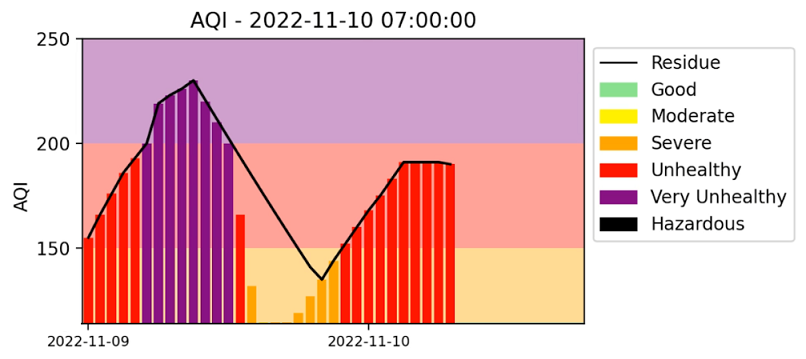
\includegraphics[width=\linewidth]{img/video.PNG}
  \label{fig:video}
\end{figure}



\section{Testing}
\subsection{Test su dispositivi}
In seguito allo sviluppo, l'applicativo è stato testato su diversi browser installati su diversi dispositivi.
I browser utilizzati sono stati Chrome, Opera, Safari e Brave, utilizzati su dispositivi Android, iOS, Windows e Linux.
Sono stati effettuati test da personal computer, smartphone e tablet di diverse risoluzioni.
In Figura \ref{fig:mobile} viene mostrata la schermata responsiva mobile su IPhone SE.

\begin{figure}[h]
  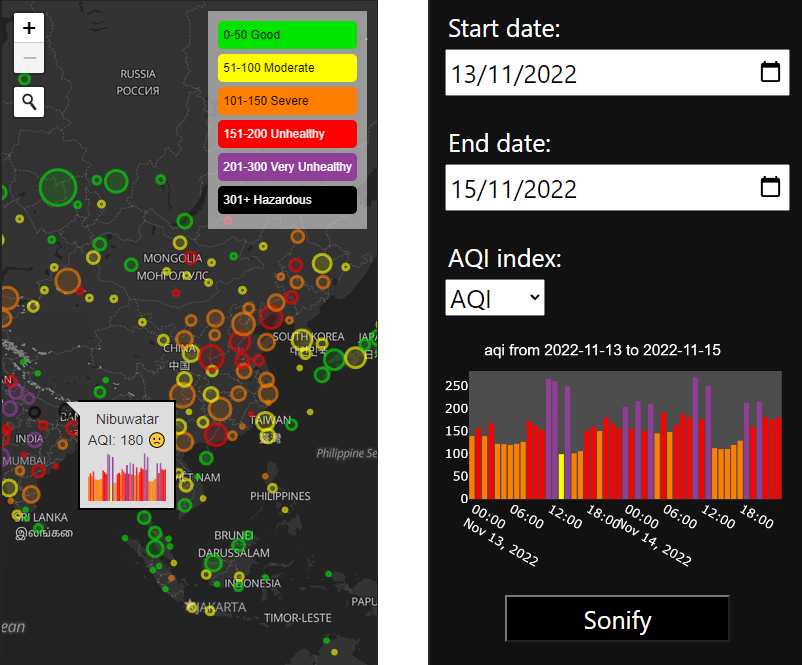
\includegraphics[width=\linewidth]{img/mobile.png}
  \label{fig:mobile}
  \caption{La schermata principale su IPhone SE.}
\end{figure}

\subsubsection{Problemi riscontrati}
Durante il test su dispositivi iOS, ho riscontrato dei problemi riguardanti la riproduzione del video.
In particolare, nonostante questo fosse visualizzato correttamente, era privo di suono.
Il problema è stato individuato visualizzando file di diversi formati su browser, questo riguardava l'incopatibilità della codifica video da parte del dispositivo.
Per risolvere questo problema, ho deciso di non utilizzare più la libreria moviepy, e di richiamare direttamente ffmpeg per unire audio e animazione.
Un secondo problema riscontrato riguardava sempre l'assenza dell'audio sul browser Brave. Il problema è stato risolto disabilitando la funzione di auto riproduzione del video. 

\subsection{Questionario SUS}
SUS (System Usability Scale) è un questionario di valutazione, sviluppato da John Brooke nel 1986 \cite{sussurvey}.
Grazie alla sua semplicità ed efficacia, è stato nominato standard internazionale per la valutazione dell'usabilità di sistemi informatici.
La formula SUS è composta da 10 domande, i cui punteggi vanno da 1 a 5; le domande riguardano principalmente la facilità d'uso, la comprensione e la soddisfazione dell'utente.

\subsubsection{Domande del questionario}
Il questionario alterna domande positive e negative, per differenziare il feedback dell'utente.
Di seguito, vengono riportate le domande del questionario, tradotte in italiano.
\begin{enumerate}
  \item Penso che mi piacerebbe utilizzare questo sistema più frequentemente;
  \item Ho trovato il sistema troppo complesso senza che ce ne fosse il bisogno;
  \item Ho trovato il sistema semplice da utilizzare;
  \item Sento il bisogno di assistenza nell'utilizzo del sistema;
  \item Ritengo che le varie funzioni del sistema siano state ben integrate;
  \item Ho riscontrato troppe inconsistenze nel sistema;
  \item Ritengo che gran parte delle persone siano in grado di utilizzare il sistema;
  \item Ho trovato il sistema macchinoso da utilizzare;
  \item Ho provato confidenza nell'utilizzo del sistema;
  \item Dovrei imparare troppe cose prima di utilizzare il sistema al meglio.
\end{enumerate}

\subsubsection{Calcolo del punteggio}
I passi per il calcolo del punteggio SUS sono i seguenti:
\begin{enumerate}
  \item Si sommano i punteggi delle domande dispari, e gli si sottrae 5;
  \item Si sommano i punteggi delle domande pari, e gli si sottrae 25;
  \item La somma di questi due numeri ottenuti viene moltiplicata per 2.5, in modo da ottenere un numero compreso tra 0 e 100.
\end{enumerate}
Per avere un riscontro immediato sul punteggio ottenuto, è possibile consultare Figura \ref{fig:sus}:

\begin{figure}[h]
  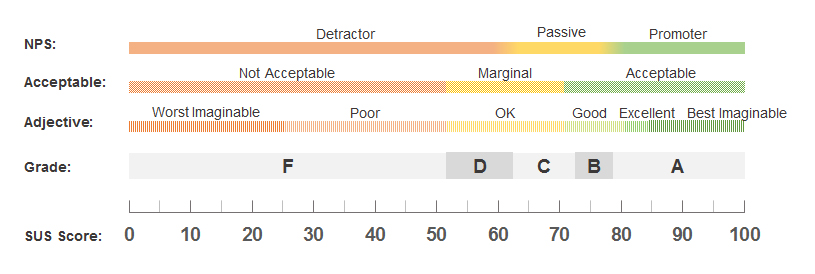
\includegraphics[width=\linewidth]{img/sus.jpg}
  \caption{Tabella con i punteggi SUS \cite{sus}.}
  \label{fig:sus}
\end{figure}

\subsubsection{Punteggio totalizzato}
Dopo avere utilizzato l'applicativo per un breve periodo di tempo, il questionario è stato compilato da 12 utenti.
Questi sono 6 compagni di corso, 4 studenti di un altro corso di studio e 2 conoscenti non particolarmente pratici di sistemi informatici.
L'età media degli utenti è di 22 anni, 10 sono di sesso maschile e 2 di sesso femminile.
Il punteggio ottenuto è stato di 89.5, somalente un campione ha riportato un punteggio inferiore a 80.
La fase di open beta ha permesso di raccogliere feedback e suggerimenti da parte degli utenti, sottolineando eventiali aspetti da migliorare.
I risultati ottenuti sono riportati in Figura \ref{fig:result}, le colonne rappresentano le risposte medie alle domande, i cui indici sono gli stessi riportati precedentemente; le domande positive sono colorate di blu, mentre quelle negative di rosso.

\begin{figure}[h]
  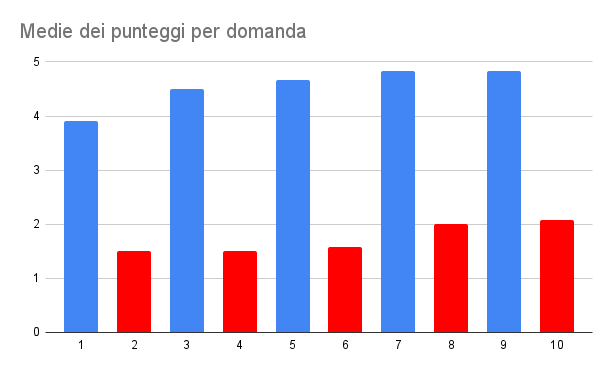
\includegraphics[width=\linewidth]{img/media.png}
  \caption{I risultati del sondaggio.}
  \label{fig:result}
\end{figure}
